\section{Markov链与概率}

我们现在看一个重要的问题, 即Markov链. 如果我们把现实生活看做状态随时间的依次推演, 那么我们自然希望通过当前的状态推知未来的状态. 这里, 我们做简化: 也就是让下一个时刻处于什么状态仅仅由当前在什么状态决定. 

\begin{definition}
    如果$E$是一个有限集或可数的无限集, 一个取值为$E$的随机变量序列$\{X_n,n\geq 0\}$是Markov链, 如果对于任何非负整数列$t_1< t_2< \cdots< t_{n}<t_{n+1}$, 以及$E$中的元素$i_1, i_2, \cdots , t_{n+1}$均成立如下的等式: 
    $$
    P(X_{t_{n+1}}=i_{n+1} | X_{t_1}=i_1, \cdots, X{_{t_n}}=i_n)=P(X_{t_{n+1}}=i_{n+1}|X_{t_n}=i_n).
    $$
    当$P(X_{t_1}=i_1, \cdots, X_{t_n}=i_n)\geq 0$. 
\end{definition}

这样的一个定义就表明, 状态$X_t$仅仅由$X_{t-1}$决定, 并且并不由$X_{t-2}$等等的历史因素决定. 这个性质叫做Markov性质或者无记忆性. 换句话说, $X_{t-1}$已经足够告诉我们$X_t$有多少概率会走向哪里了. 

不失一般性, 我们可以令集合$E$为$\{0,1,2,\cdots, n\}$. 下面, 我们自然希望得到从一个状态转移到另一个状态的概率是多少. 比如我现在在$i$状态, 下一个时刻可能在$j$的概率
$$
P_{i,j}:=P(X_t=j|X_{t-1}=i).
$$

如果我们把所有的可能的转移都画出来, 也就是$P_{0,0}, P_{0,1}, \cdots, P_{n,n}$, 就构成了一个矩阵. 我们把它叫做转移矩阵. 用$\bf P$表示.
$$
\mathbf{P}=\left(\begin{array}{ccccc}P_{0,0} & P_{0,1} & \cdots & P_{0, j} & \cdots \\ P_{1,0} & P_{1,1} & \cdots & P_{1, j} & \cdots \\ \vdots & \vdots & \ddots & \vdots & \ddots \\ P_{i, 0} & P_{i, 1} & \cdots & P_{i, j} & \cdots \\ \vdots & \vdots & \ddots & \vdots & \ddots\end{array}\right)
$$

根据上面的描述, 我们会发现这个矩阵满足对于任意的$i$, 有$\sum_{j\geq 0}P_{i,j}=1$. 我们把这个写作矩阵形式, 最方便的一点就是: 在我们经过了很多次迭代之后, 问一问到达每一个状态的概率会稳定吗? 如果稳定, 那么大概是多少? 如果可以稳定的话, 它就称作稳定状态. 下面我们来看一看如何得到稳定状态. 

令$p_i(t)$表示在时刻$t$在状态$i$的概率. 把时刻$t$的每一个状态收集到一个向量里面, 就有$\vec{p}(t):=\left(p_0(t), p_1(t), p_2(t), \ldots\right)$. 那么, 要从$t-1$时刻的分布向量$\vec{p}(t-1)$得到$t$时刻的分布向量, 根据这次只与上次相关的性质, 就有对于每一个可能转移过来的状态, 乘上从上个时刻转移到这个时刻的概率, 也就是$$p_i(t)=\sum_{j \geq 0} p_j(t-1) P_{j, i},$$ 为了方便起见, 使用矩阵的形式写出来: $$\vec{p}(t)=\vec{p}(t-1) \mathbf{P}.$$

所以我们现在知道了从上一时刻到这一时刻的时候概率的变化. 下面, 我们来定义从$i$到$j$, 经历了$m$步, 停在某一个状态的概率: 
$$
P_{i, j}^m:={P}\left(X_{t+m}=j \mid X_t=i\right)
$$
把上面的行向量拼起来, 对于每一行施以同样的操作, 我们就有$$P_{i, j}^m=\sum_{k \geq 0} P_{i, k} P_{k, j}^{m-1}. $$ 这时候, 我们就需要依赖经历了$m-1$步的基础上面再走一步. 

如果我们使用矩阵的记号进行表述的话, 就会有更神奇的. 令$\mathbf{P}^{({m})}$表示经过$m$步转移之后的概率. 这个矩阵中的每一项就表示
$P_{i, j}^{\bf{m}}$, 这时候把上面的求和号的式子改写为矩阵的形式, 就有: 
$$
\mathbf{P}^{(\bf {m})}=\mathbf{P} \cdot \mathbf{P}^{(\bf {m}-1)} ;
$$
如果我们对它施以归纳法, 就得到了$$
\mathbf{P}^{(\mathbf{m})}=\mathbf{P}^{{m}}.
$$
这就表明对于任意的$t\geq 0, m\geq 1$, 有
$$
\vec{p}(t+m)=\vec{p}(t) \mathbf{P}^{{m}}
$$

我们可以使用带权重的有向图(可能有自环)$D=(V,E,w)$来表示Markov链的转移过程. 节点表示状态, 节点与节点之间的边就表示了从一个状态转移到另一个状态的概率. 更具体地说, 如果我们有一条边$(i,j)\in E,$其权重为$w(i,j)=P_{i,j}$. 根据上面的描述, 每个出边的权重和必须为1, 也就是$\sum_{j:(i, j) \in E} w(i, j)=1$. 比如\cref{fig:markov-chain-graph}所示的就是右侧的概率转移矩阵的一个图像化的表示. 

\begin{figure}
    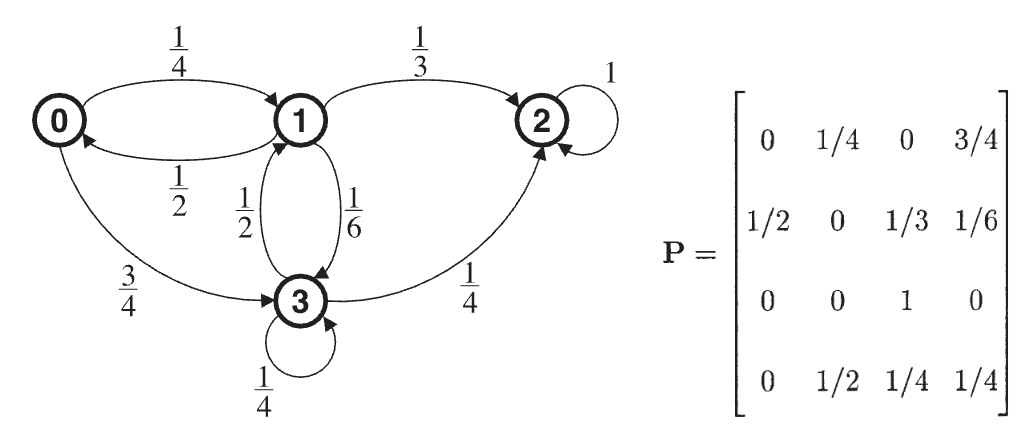
\includegraphics[width=0.8\textwidth]{fig/ch6/markov.jpg}
    \caption{一个Markov链的例子}
    \label{fig:markov-chain-graph}
\end{figure}

\begin{example}
    在\cref{fig:markov-chain-graph}中, 我们发现从状态0到状态3一共有如下的几种形态: $0\to 1\to 0\to 3,0\to 1\to 3\to 3,0\to 3\to 1\to 3$,以及 $0\to 3\to 3\to 3$. 它们的概率分别是$3 / 32,1 / 96,1 / 16$, 和 $3 / 64$. 把它们加起来, 总共的可能性是$41/192$. 实际上, 我们可以直接计算转移矩阵$\bf P$的$3$次方. 也就是
    $$\mathbf{P}^3=\left[\begin{array}{cccc}3 / 16 & 7 / 48 & 29 / 64 & 41 / 192 \\ 5 / 48 & 5 / 24 & 79 / 144 & 5 / 36 \\ 0 & 0 & 1 & 0 \\ 1 / 16 & 13 / 96 & 107 / 192 & 47 / 192\end{array}\right]$$
    我们发现这个矩阵的$P_{0,3}^3=41 / 192$给出了我们正确的答案. 如果我们已经知道了初始状态下, 处于每一个点的概率是均等的(都是$1/4$), 我们就可以得到在这个分布条件下最后到达每个节点的概率. 也就是: 
    $$(1 / 4,1 / 4,1 / 4,1 / 4) \mathbf{P}^3=(17 / 192,47 / 384,737 / 1152,43 / 288).$$
\end{example}